% !TeX root = ../main.tex
% Add the above to each chapter to make compiling the PDF easier in some editors.

\chapter{Experiments}\label{chapter:experiments}

This chapter presents the experiments conducted within the thesis and describes the key design choices
and the motivation behind each campaign.
Detailed results and metric comparisons are evaluated in \autoref{chapter:results}.

\section{Experimental Infrastructure}\label{sec:infra}

To ensure reproducibility, the whole pipeline runs within a Docker environment.
The pipeline includes distinct scripts for data generation, model training and model evaluation.
The training data is stored in HDF5 file format to enable fast access, and is shared across experiments unless stated otherwise.
Its generation was performed on an AMD Ryzen AI 7 350 and an AMD Ryzen 5 1600 Six-Core, described in more detail in \autoref{sec:dataset}
Checkpoints and logs are namespaced by experiment name and image size, allowing multiple runs to coexist without overwriting.
The training of the model for the different experiments was done on an NVIDIA GeForce RTX 5060 Laptop GPU.
All runs use a fixed random seed for reproducibility.
No special CPU configurations were done during data generation, since all solvers for a given matrix are benchmarked sequentially in the same process, core allocation variability affects their timings equally for a given matrix.
However, absolute timings and winner assignments remain hardware-dependent, and parallel solver configurations in particular may produce different results on machines with different core counts or memory layouts.

The full source code, configuration files, experiment logs and LaTeX sources that were used for the thesis are publicly available on GitHub\footnote{\url{https://github.com/Draggon01/IterativeSolverSelectionWithCNNs}} within the \texttt{Thesis-Submission} release marks the exact repository state at hand-in.

\section{Evaluation Metrics}\label{sec:metrics}

\subsection{Classification Metrics}\label{subsec:classification-metrics}

The experiment results are measured with four classification metrics, following the evaluation protocol of MM-AutoSolver~\cite{xiong2025mmautosolver}, to allow direct comparison:

\begin{itemize}
  \item \textbf{Accuracy (Acc)} - the fraction of test samples for which the predicted solver-preconditioner pair matches the best solver.
  \item \textbf{Macro Precision (MP)} - the average per-class precision across all 19 classes, weighted equally regardless of class size.
  \item \textbf{Macro Recall (MR)} - the average per-class recall, weighted equally across all classes.
  \item \textbf{Macro F1 (F1)} - the harmonic mean of macro precision and macro recall, balancing both measures into a single score.
\end{itemize}

Macro averaging is used rather than weighted averaging to treat all solver classes equally, which is important given the imbalanced class distribution in the dataset.

\subsection{Solver-Quality Metrics}\label{subsec:solver-quality-metrics}

If a predicted solver-preconditioner pair is not the best result but comes in as a close second, it will not be recognised
for the accuracy, which may not be ideal when targeting the implementation of the models within a specific pipeline.
For this case four additional metrics are introduced, which also give positive feedback if the chosen solver-preconditioner
pair is only marginally slower, just the second-best choice, or is extremely failure-resistant.

\begin{itemize}
    \item \textbf{Top-k accuracy (k=2,3)} - probability the predicted solver is within the top-k predictions. Top-3 accuracy is used as the primary quality metric in the results discussion, with near-optimal values available in the experiment summary files.
    \item \textbf{Near-optimal accuracy (k=5,10,20)} - the predicted solver is within k\% of the best solver time.
    \item \textbf{Mean Runtime Ratio (MRT×)} - the average ratio of the predicted solver's runtime to the best solver's runtime. A value of 1.0 means the predicted solver is always optimal; higher values indicate how much slower the predictions are on average. Samples where the predicted solver did not converge are excluded from the MRT calculation and counted in the failure rate instead, so the two metrics should be read together.
    \item \textbf{Failure rate} - the fraction of test samples where the predicted solver did not converge. This matters in practice because a non-converging solver must run to timeout before the failure is detected, which can be more costly than simply picking a slower but converging solver.
\end{itemize}

\subsection{Computational Cost}\label{subsec:compute-cost}

Training time and per-matrix inference cost (feature extraction and image rendering) are also recorded for each experiment.
Data generation time was not tracked.
These are reported in \autoref{chapter:results} alongside the classification metrics.

\subsection{Non-Learning Baselines}\label{subsec:baselines}

Two non-learning baselines are introduced as reference points.
\textbf{1-NN} and \textbf{5-NN} are $k$-nearest-neighbour classifiers that predict the best solver
by finding the most similar training matrices in the scalar feature space
(14-dimensional in Campaigns~1 and~3, 20-dimensional in Campaigns~2 and~4), without any CNN branch.
Additionally, a \textbf{nocnn} baseline disregards the CNN branch entirely,
learning only from the feature vector through the MLP and classification head.
This is used to isolate the contribution of the image input and allows the CNN's
value to be assessed independently of the feature branch.

\section{MM-AutoSolver Replication}\label{sec:mm-replication}

The first experiment replicates the results of the MM-AutoSolver~\cite{xiong2025mmautosolver} paper with a dataset that resembles the
dataset from the paper in solver-preconditioner distribution.
Due to the high computational cost of the benchmarking process for the 19 solver-preconditioner pairs that also scales significantly with matrix size,
the replication dataset is limited to matrices with up to 84{,}617 rows, compared to over one million rows in the original paper.
Table~\ref{tab:replication-distribution} compares the per-class sample counts of the replication dataset against the actual numbers of the paper.

Since the generator buckets were less targeted in the early stages, generation of certain classes took a significant amount of time.
Therefore, different classes are over- and underrepresented and the dataset remains skewed, but in different directions than the paper.

\begin{table}[H]
  \centering
  \caption{Per-class sample counts: MM-AutoSolver paper dataset vs.\ replication dataset used in this thesis.}
  \label{tab:replication-distribution}
  \begin{tabular}{lrrrr}
    \toprule
    \textbf{Solver} & \textbf{Ours} & \textbf{Ours\,\%} & \textbf{Paper} & \textbf{Paper\,\%} \\
    \midrule
    \texttt{fbcgsr+jacobi} & 2519 & 10.9 & 2173 & 18.7 \\
    \texttt{bcgsl+none}    & 2502 & 10.8 & 2054 & 17.7 \\
    \texttt{symmlq+icc}    &  162 &  0.7 & 1201 & 10.3 \\
    \texttt{symmlq+jacobi} &  211 &  0.9 &  923 &  7.9 \\
    \texttt{dgmres+none}   &   43 &  0.2 &  650 &  5.6 \\
    \texttt{gmres+gamg}    &  394 &  1.7 &  640 &  5.5 \\
    \texttt{cr+eisenstat}  & 2505 & 10.8 &  598 &  5.1 \\
    \texttt{symmlq+sor}    &  109 &  0.5 &  582 &  5.0 \\
    \texttt{fbcgsr+ilu}    & 1247 &  5.4 &  562 &  4.8 \\
    \texttt{minres+gamg}   &  412 &  1.8 &  524 &  4.5 \\
    \texttt{fcg+gamg}      &  143 &  0.6 &  342 &  2.9 \\
    \texttt{cr+jacobi}     & 2503 & 10.8 &  310 &  2.7 \\
    \texttt{cg+ilu}        & 2511 & 10.8 &  275 &  2.4 \\
    \texttt{fgmres+gamg}   &  146 &  0.6 &  226 &  1.9 \\
    \texttt{cg+eisenstat}  & 2525 & 10.9 &  224 &  1.9 \\
    \texttt{cg+bjacobi}    & 2503 & 10.8 &  193 &  1.7 \\
    \texttt{cr+ilu}        & 2500 & 10.8 &   68 &  0.6 \\
    \texttt{cgs+gamg}      &  106 &  0.5 &   49 &  0.4 \\
    \texttt{bcgsl+asm}     &  126 &  0.5 &   29 &  0.2 \\
    \midrule
    Total                  & 23{,}167 & 100.0 & 11{,}623 & 100.0 \\
    \bottomrule
  \end{tabular}
\end{table}

Figure~\ref{fig:replication-sizes} shows the distribution of matrix sizes in the replication dataset,
with sizes ranging from 100 to 84{,}617 rows and a median of 1{,}485.

\begin{figure}[H]
  \centering
  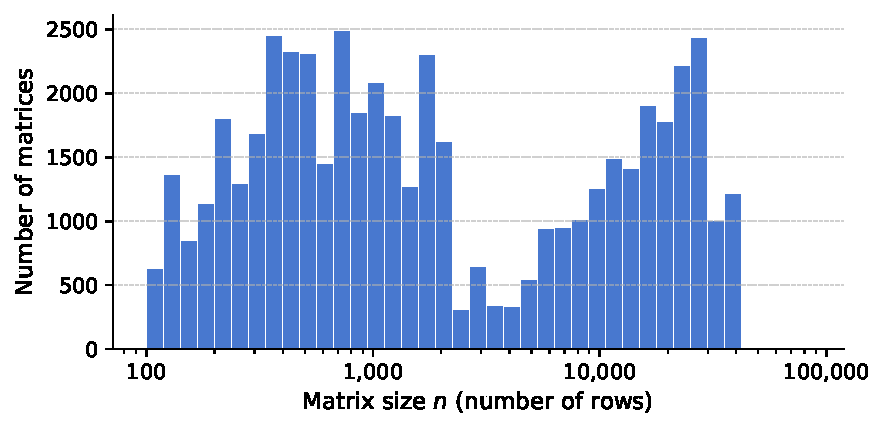
\includegraphics[width=0.85\textwidth]{figures/replication_size_histogram.pdf}
  \caption{Distribution of matrix sizes (number of rows $n$) for the MM-AutoSolver replication dataset
           (23{,}167 matrices). The $x$-axis uses a logarithmic scale.}
  \label{fig:replication-sizes}
\end{figure}

Following the paper, the experiment uses a $128 \times 128$ pixel density image for the CNN branch
and the 17 features proposed in the original work.
The re-implementation uses the original MM-AutoSolver architecture, two convolutional layers with Tanh activation
and element-wise CNN/MLP fusion, rather than the thesis model~(\autoref{sec:architecture}).
For the training, a learning rate of $10^{-3}$, $256$ training epochs and a batch size of $512$ are set.

\section{Single-Channel Experiments}\label{sec:single-channel-exp}

This section describes the different experiments done with a single CNN channel active.
They differ in their feature vector, the activation of the non-convergence penalty and model size.

\subsection{Campaign 1: Single-Channel Baseline}\label{subsec:campaign1}

The first experiment on the single branch is used to create a baseline for future experiment runs.
The 14 different image modes~(\autoref{sec:image-modes}) are tested to determine which of them carries the most useful information, and they are run on both 64\,px and 128\,px images.
Convergence penalty is deactivated and the small model~(\autoref{sec:architecture}) is used to establish a clean baseline.

\subsection{Campaign 2: Extended Features and Convergence Penalty}\label{subsec:campaign2}

Campaign 2 addresses two weaknesses observed in Campaign 1.
Some solvers had especially low accuracy and F1 values. An additional 6 features described in \autoref{tab:features-6} were therefore introduced.
To reduce high failure rates observed in certain classes, the convergence penalty~(\autoref{sec:training}) with $\lambda = 1.0$ is used.
The whole experiment is run on the large model~(\autoref{sec:architecture}) and uses the same image modes as Campaign 1 but only an image size of 64\,px.

\section{Dual-Channel Experiments}\label{sec:dual-channel-exp}

This section describes the experiments that use the dual-channel CNN approach.
To reduce computation time, only the best single-channel approach modes are combined with additional combinations included where
mode pairs are expected to capture complementary matrix information.

\subsection{Multimode HDF5 and Rendering Pipeline}\label{subsec:multimode-hdf5}

To evaluate dual-channel experiments efficiently, all required image modes are pre-rendered into a single shared HDF5 file
rather than maintaining separate per-experiment datasets.
The file stores one dataset per image mode under the key \texttt{images\_<mode>}, alongside the shared features, labels and runtimes from the original dataset.

\subsection{Campaign 3: Dual-Channel Approach}\label{subsec:campaign3}

The experiment setup is similar to the one in Campaign 1, except this time a different set of image modes and the large model~(\autoref{sec:architecture}) are used and
the image sizes are fixed at 64\,px.
Six image modes are selected from Campaign~1~(\autoref{subsec:campaign1}) based on F1 score and complementary information content, together with the sign mode.
These 7 methods are then combined into all their pairwise combinations and tested.
This results in 21 different image mode combinations that can be seen in Table~\ref{tab:results-campaign3}.

\subsection{Campaign 4: Dual-Channel with Extended Features}\label{subsec:campaign4}

This campaign combines the dual-channel approach with the improvements introduced in Campaign~2~(\autoref{subsec:campaign2}) with convergence penalty $\lambda = 1.0$, the 20-feature set and the large model~(\autoref{sec:architecture}).
The image modes are selected based on F1 performance in Campaign 2, and all selected mode pairs are run on both 64\,px and 128\,px.
This results in 15 different image mode combinations each run at two image sizes, giving 30 models in total.

\section{Ensemble Evaluation}\label{sec:ensemble}

\subsection{Campaign 5: Ensemble Method}\label{subsec:ensemble-method}

The ensemble combines independently trained models by averaging their predicted class probabilities before taking the final prediction.
No retraining is required as the member models are loaded from their saved checkpoints and are
evaluated on the shared validation split.

The shared multimode HDF5 (\autoref{subsec:multimode-hdf5}) ensures that all members
receive identical image data during ensemble inference.
Member selection follows two criteria: high individual F1 and complementary second
channels, so that the ensemble covers a wider range of matrix characteristics than
any single model.

For Campaign~3 the four ensemble members are (all 64\,px):
\begin{itemize}
  \item \texttt{magnitude+signed\_magnitude}
  \item \texttt{magnitude+rcm\_signed\_magnitude}
  \item \texttt{magnitude+symmetry}
  \item \texttt{rcm\_magnitude+signed\_magnitude}
\end{itemize}

For Campaign~4 the evaluated ensemble uses four members (all 128\,px):
\begin{itemize}
  \item \texttt{magnitude+log\_density}
  \item \texttt{magnitude+rcm\_log\_density}
  \item \texttt{rcm\_magnitude+rcm\_signed\_magnitude}
  \item \texttt{symmetry+log\_density}
\end{itemize}
These were selected for complementary first channels (magnitude $\times$2, \texttt{rcm\_magnitude}, symmetry)
and non-redundant second channels.

